\documentclass[12pt]{report}
\usepackage{amssymb}
\usepackage{amsmath}

\usepackage{multicol}
\usepackage{graphicx}
\usepackage{subfigure}
\usepackage{verbatim}

%\usepackage{adjustbox}

\usepackage[letterpaper,left=1cm,right=2cm, top=1.5cm,
bottom=1.5cm,head=0cm,foot=1cm]{geometry}

\parindent=0in


\newcommand{\m}{\mbox{m}}
\newcommand{\kg}{\mbox{kg}}
\newcommand{\s}{\mbox{s}}
\newcommand{\ke}{\mbox{\small KE}}
\newcommand{\pe}{\mbox{\small PE}}
\newcommand{\net}{\mbox{\tiny net}}


\newcommand{ \probDir}[1]{{ \bf\small #1 \mbox{  }}}



\newcommand{ \breakList}{\setcounter{saveenum}{\value{enumi}} \end{enumerate}}
\newcommand{ \contList}{\begin{enumerate} \setcounter{enumi}{\value{saveenum}}}

\newcounter{saveenum}

\def \wspace{5cm}

%%%%%%%%%%%%%%%%%%%%%%%%%%%%%%%%%%%%%%%%%
\begin{document}

{\bf{Honors Physics} \hfill Example: Mass on a Clothesline \hfill {Mr. Kelley}} \\ \\
%%%%%%%%%%

\vspace{1cm}

\hspace{1.5cm} \parbox{12 cm}{Suppose there is a 12 kg mass hanging at the center of a clothesline.  The mass is at rest.  The clothesline is depressed by an angle of $15^{\circ}$ with respect to the horizontal?  What is the tension in the two halves of the clothesline?}  \\
\vspace{1cm}

\hfill \raisebox{-0cm}{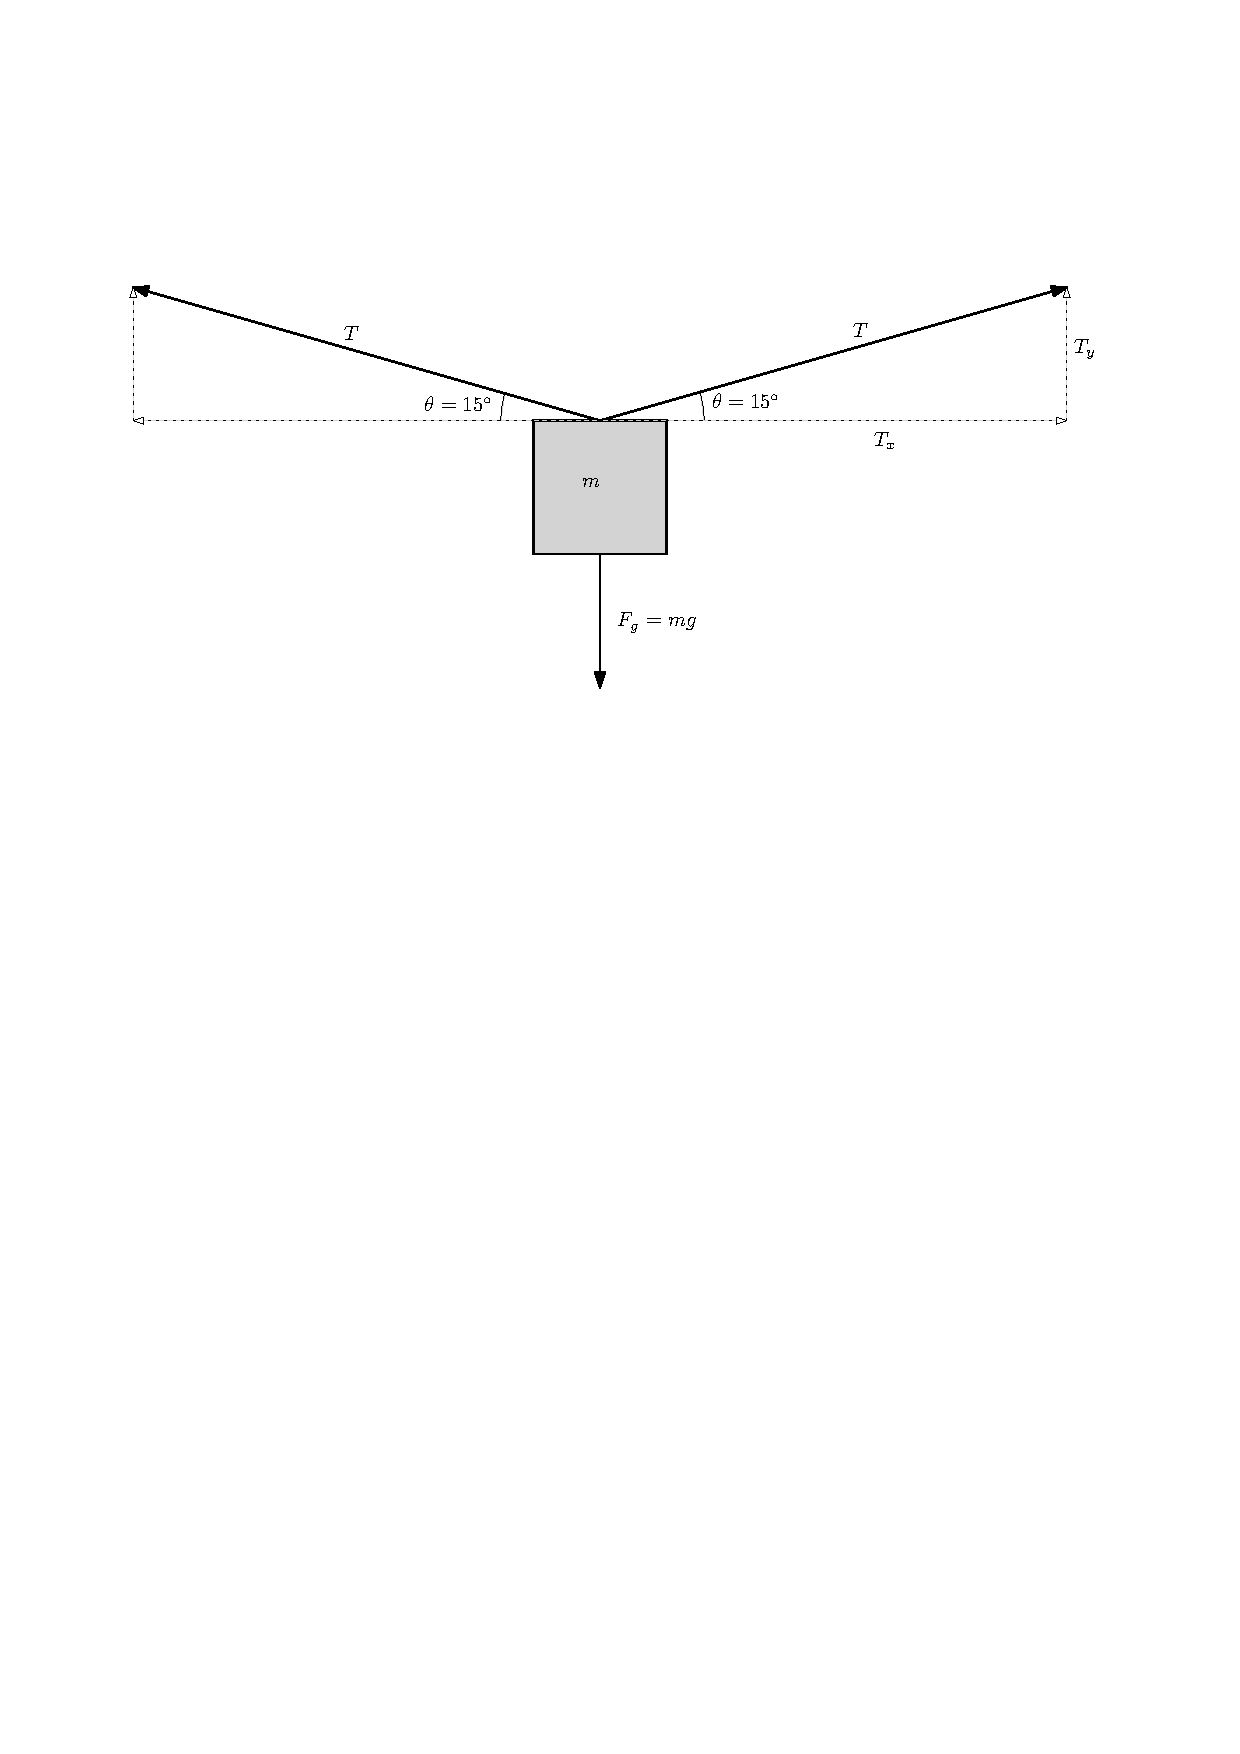
\includegraphics[scale = 1.1]{massClothesline}} \hfill \mbox{} \\

\raisebox{0cm}{\parbox[t]{7cm}{We know that the mass is at rest, so $F_{\net} = 0$.  That means $F_{\net x} = 0$ and $F_{\net y} = 0$.}} \hfill \raisebox{0cm}{\parbox[t]{7cm}{$$\sum F_y = T_y+T_y - F_g = 0$$  $$2T_y - mg = 0$$ $$T_y = \frac{mg}{2}$$}}

\raisebox{2cm}{\parbox[t]{9cm}{We can see that the $T_x$'s are equal and in opposite directions ($\sum F_x= 0$).  To find them we just use $\tan\theta$ since we already know $T_y$.  $$\tan\theta = \frac{T_y}{T_x} \Longrightarrow T_x = \frac{T_y}{\tan\theta}$$ $$T_x = \frac{mg}{2\tan\theta}$$}} \hfill \parbox[t]{8cm}{To find the magnitude of T, use the pythagorean theorem: $$T = \sqrt{T_x^2 + T_y^2}$$} \\

\vspace{1cm}
\parbox{8cm}{Compute values for $F_g$ and $T$:}

\pagebreak

\hspace{3cm} \parbox{12 cm}{Now suppose the 12 kg mass hanging \emph{off}-center on a clothesline.  The mass is at rest.  The clothesline is depressed by an angle of $25^{\circ}$  on one side and $12^{\circ}$ on the other, with respect to the horizontal.  What is the tension in the two halves of the clothesline?}  \\
\vspace{1cm}

\hfill \raisebox{-0cm}{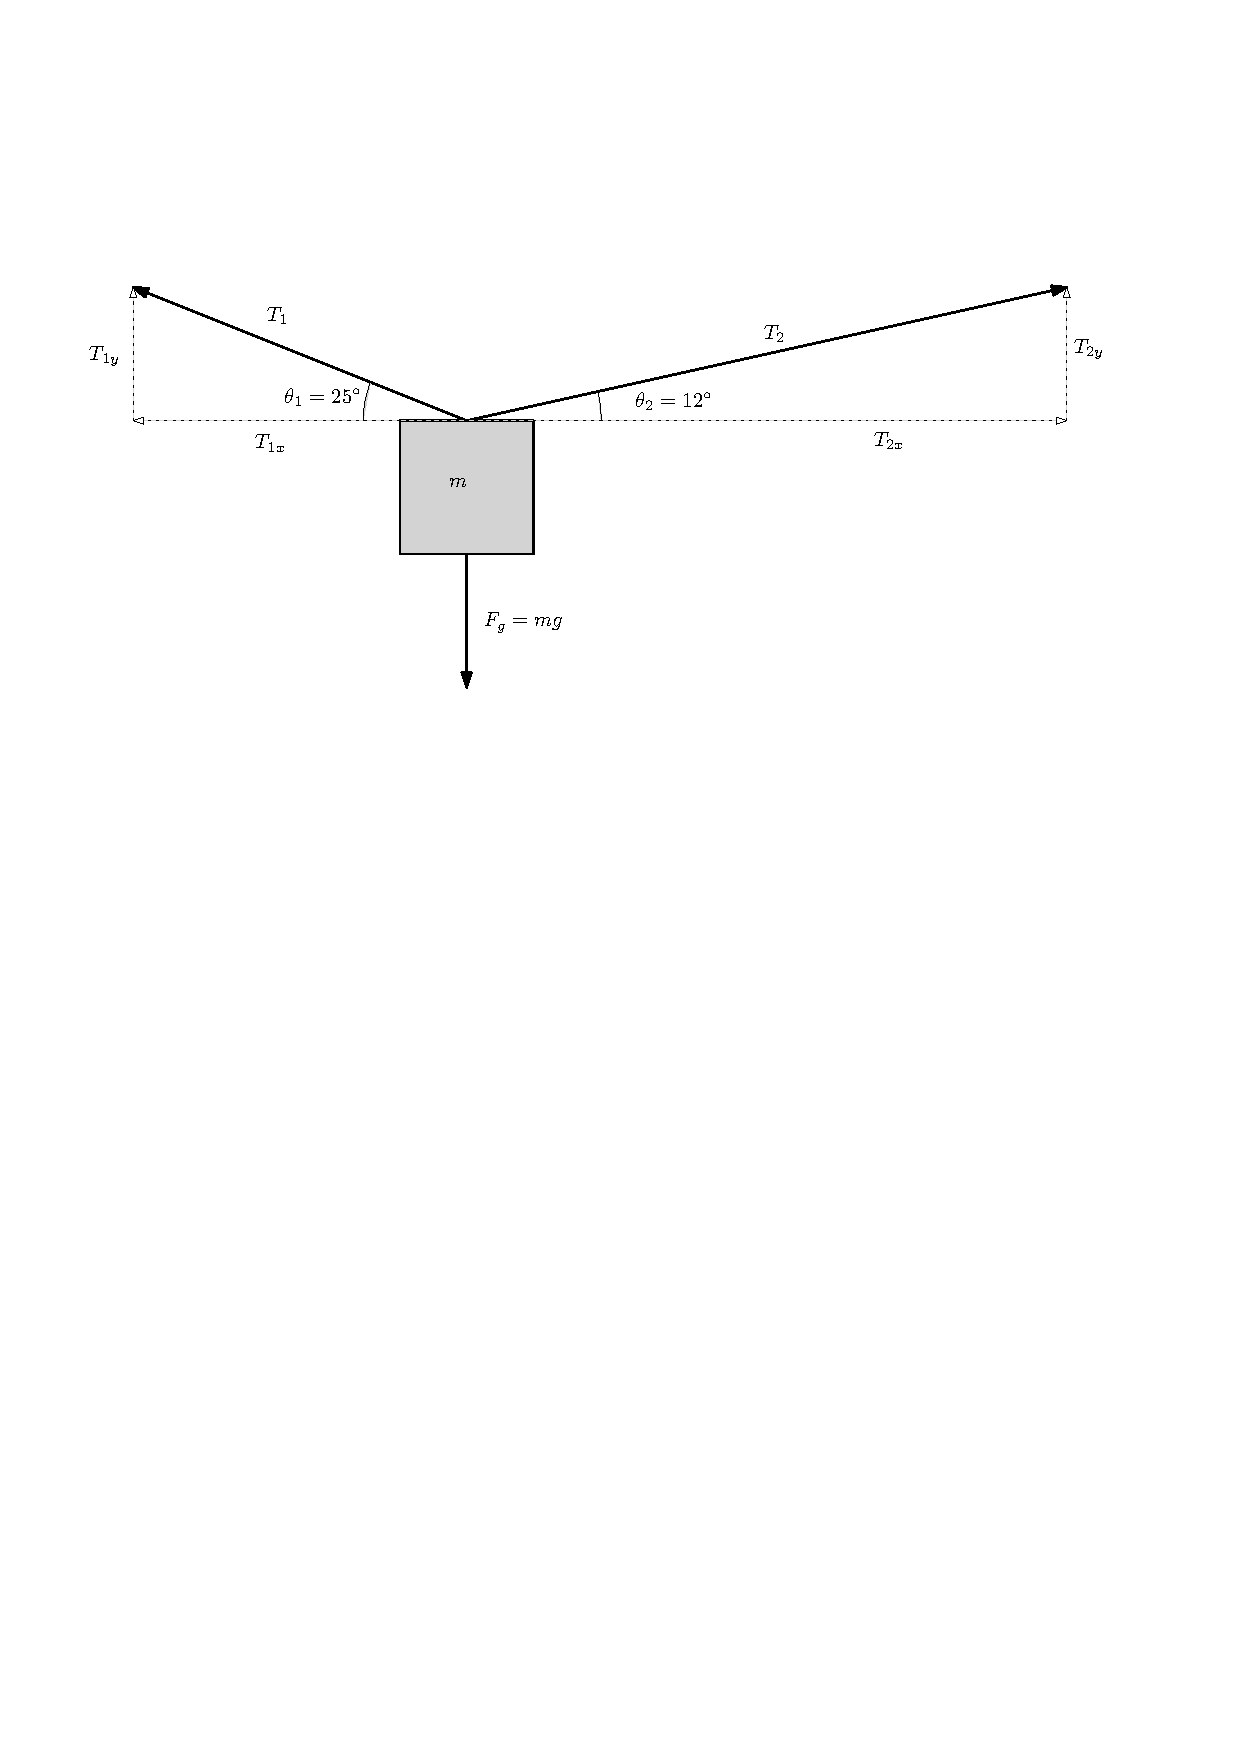
\includegraphics[scale = 1.1]{massClotheslineOffCenter}} \hfill \mbox{} \\

\raisebox{0cm}{\parbox[t]{7cm}{\centering Just like before: \\ \vspace{.3cm} $\sum F_x= 0$ and $\sum F_y= 0$}} \hfill \fbox{\parbox[t]{7cm}{$$\sum F_y = T_{1y}+T_{2y} - F_g = 0$$  $$T_{1y} + T_{2y} = F_g$$ \hrule $$\sum F_x = -T_{1x}+T_{2x}  = 0$$ $$T_{1x} = T_{2x}$$}}

\vspace{.5cm}

\parbox[t]{9cm}{What we end up with is a system of equations: \vspace{1cm} $$T_1\sin{\theta_1} + T_2 \sin{\theta_2} = mg$$  $$T_1 \cos\theta_1 = T_2 \cos\theta_2$$} \hspace{1cm} \parbox[t]{6cm}{\centering Use substitution: $$T_1   = T_2 \frac{\cos\theta_2}{\cos\theta_1}$$ $$T_2 \frac{\cos\theta_2}{\cos\theta_1} \sin{\theta_1} + T_2 \sin\theta_2 = mg$$ \vspace{.2cm} $$T_2(\cos\theta_2 \tan\theta_1 + \sin{\theta_2}) = mg$$ \vspace{.1cm} $$T_2 = \frac{mg}{\cos\theta_2 \tan\theta_1 + \sin{\theta_2}}$$} \hfill

\vspace{1cm}

\parbox[t]{6cm}{Compute the values for $T_1$ and $T_2$:} 


\end{document}